\documentclass[twocolumn,a4j]{jarticle}
\usepackage[dvipdfmx]{graphicx}
\usepackage{url}
\usepackage{ascmac}
\usepackage{amsmath, amssymb}
\usepackage{fancyhdr}
\usepackage{tikz}
\usepackage{multirow}
\usepackage{adjustbox}
\usepackage{graphicx} 
\usepackage{enumitem}
\renewcommand{\topfraction}{1.0}
\renewcommand{\bottomfraction}{1.0}
\renewcommand{\dbltopfraction}{1.0}
\renewcommand{\textfraction}{0.01}
\renewcommand{\floatpagefraction}{1.0}
\renewcommand{\dblfloatpagefraction}{1.0}
\setcounter{topnumber}{5}
\setcounter{bottomnumber}{5}
\setcounter{totalnumber}{10}

% 所属と氏名を右寄せにする設定
\makeatletter
  \def\@maketitle{%
  \newpage\null
  %\vskip 2em%
  \begin{center}%
  \let\footnote\thanks
    {\LARGE \@title \par}%
    %\vskip 1.5em%
  \end{center}% 追加
  \begin{center}% 追加
    {\large \@author}%
  \end{center}%
    %\mbox{}\hfill%% 追加
    %{\large
      %\lineskip .5em%
      %\begin{tabular}[t]{r}%
        %\@author
      %\end{tabular}\par}%
    %\vskip 1em%
  \begin{center}% 追加
    {\large \@date}%
  \end{center}%
  %\par\vskip 1.5em
}
\makeatother
\def\vec#1{\mbox{\boldmath $#1$}} 


% 余白の設定
\usepackage[top=20truemm,bottom=20truemm,left=25truemm,right=15truemm]{geometry}


% 箇条書きの行間
\let\olditemize\itemize
\renewcommand{\itemize}{
\olditemize
\setlength{\itemsep}{0.5pt}
\setlength{\parskip}{0pt}
\setlength{\parsep}{0pt}
}

%%%%%%%%%%%%%%%%%%%%%%%%%%%%%%%% 皆さんが書き換えるのはここから %%%%%%%%%%%%%%%%%%%%%%%%%%%%%%%%%%%%%%%

% タイトル
\title{安全運転の持続的な意識づけを促す\\運転操作フィードバック手法に関する研究}
\author{発表者:機械知能システム学専攻 北川 浩行(2332034),k2332034@edu.cc.uec.ac.jp\\
主任指導教員:中村 友昭 准教授,副指導教員:横井 浩史 教授} % 所属,学籍番号,名前
\date{}

%%%%%%%%%%%%%%%%%%%%%%%%%%%%%%%%
% ここの数字をいじってページ数をちょうど1ページに合わせましょう.
\renewcommand{\baselinestretch}{1}
%%%%%%%%%%%%%%% ここまで %%%%%%%%%%%%%%%%%

\begin{document}
\maketitle

\def\bq{\begin{equation}}
\def\eq{\end{equation}}
\def\beq{\begin{eqnarray}}
\def\eeq{\end{eqnarray}}
\def\ba{\begin{array}}
\def\ea{\end{array}}
\def\bc{\begin{center}}
\def\ec{\end{center}}
\def\dsum{\sum\limits}
\def\disp{\displaystyle}
\def\ejw{e^{j\omega}}
\def\ejwi{e^{j\omega_{i}}}
\def\e-jwi{e^{-j\omega_{i}}}
\def\dfrac#1#2{\disp{\frac{#1}{#2}}}
\def\teigi{\stackrel{\triangle}{=}}
%\def\b0{\mbox{\boldmath$0$}}
\if0
\def\baa{\mbox{\boldmath$a$}}
\def\bb{\mbox{\boldmath$b$}}
\def\bcc{\mbox{\boldmath$c$}}
\def\bd{\mbox{\boldmath$d$}}
\def\be{\mbox{\boldmath$e$}}
\def\bff{\mbox{\boldmath$f$}}
\def\bg{\mbox{\boldmath$g$}}
\def\bh{\mbox{\boldmath$h$}}
\def\bi{\mbox{\boldmath$i$}}
\def\bj{\mbox{\boldmath$j$}}
\def\bk{\mbox{\boldmath$k$}}
\def\bl{\mbox{\boldmath$l$}}
\def\bm{\mbox{\boldmath$m$}}
\def\bn{\mbox{\boldmath$n$}}
\def\bo{\mbox{\boldmath$o$}}
\def\bp{\mbox{\boldmath$p$}}
\def\bqq{\mbox{\boldmath$q$}}
\def\br{\mbox{\boldmath$r$}}
\def\bs{\mbox{\boldmath$s$}}
\def\bt{\mbox{\boldmath$t$}}
\def\bu{\mbox{\boldmath$u$}}
\def\bv{\mbox{\boldmath$v$}}
\def\bw{\mbox{\boldmath$w$}}
\def\bx{\mbox{\boldmath$x$}}
\def\by{\mbox{\boldmath$y$}}
\def\bz{\mbox{\boldmath$z$}}
\def\bA{\mbox{\boldmath$A$}}
\def\bB{\mbox{\boldmath$B$}}
\def\bC{\mbox{\boldmath$C$}}
\def\bD{\mbox{\boldmath$D$}}
\def\bE{\mbox{\boldmath$E$}}
\def\bF{\mbox{\boldmath$F$}}
\def\bG{\mbox{\boldmath$G$}}
\def\bH{\mbox{\boldmath$H$}}
\def\bI{\mbox{\boldmath$I$}}
\def\bJ{\mbox{\boldmath$J$}}
\def\bK{\mbox{\boldmath$K$}}
\def\bL{\mbox{\boldmath$L$}}
\def\bM{\mbox{\boldmath$M$}}
\def\bN{\mbox{\boldmath$N$}}
\def\bO{\mbox{\boldmath$O$}}
\def\bP{\mbox{\boldmath$P$}}
\def\bQ{\mbox{\boldmath$Q$}}
\def\bR{\mbox{\boldmath$R$}}
\def\bS{\mbox{\boldmath$S$}}
\def\bT{\mbox{\boldmath$T$}}
\def\bU{\mbox{\boldmath$U$}}
\def\bV{\mbox{\boldmath$V$}}
\def\bW{\mbox{\boldmath$W$}}
\def\bX{\mbox{\boldmath$X$}}
\def\bY{\mbox{\boldmath$Y$}}
\def\bZ{\mbox{\boldmath$Z$}}
\fi
\if0
\def\b0{\bf{0}}
\def\bPhi{\mbox{\boldmath$\Phi$}}
\def\bomega{\mbox{\boldmath$\omega$}}
\def\bLambda{\mbox{\boldmath$\Lambda$}}
\def\blambda{\mbox{\boldmath$\lambda$}}
\def\bmu{\mbox{\boldmath$\mu$}}
\def\bnu{\mbox{\boldmath$\nu$}}
\def\bSigma{\mbox{\boldmath$\Sigma$}}
\def\bPhi{\mbox{\boldmath$\Phi$}}
\def\balpha{\mbox{\boldmath$\alpha$}}
\def\bTheta{\mbox{\boldmath$\Theta$}}
\def\btheta{\mbox{\boldmath$\theta$}}
\def\bGamma{\mbox{\boldmath$\Gamma$}}
\def\bPsi{\mbox{\boldmath$\Psi$}}
\def\bDelta{\mbox{\boldmath$\Delta$}}
\def\bPi{\mbox{\boldmath$\Pi$}}
\fi
\makeatletter
\def\lddots{\mathinner{\mkern1mu\raise\p@\vbox{\kern7\p@\hbox{.}}\mkern2mu
\raise4\p@\hbox{.}\mkern2mu\raise7\p@\hbox{.}\mkern1mu}}
\makeatother
\def\argmax{\mathop{\rm argmax}}
\def\baa{{ \boldsymbol a}}
\def\bb{{ \boldsymbol b}}
\def\bcc{{ \boldsymbol c}}
\def\bd{{ \boldsymbol d}}
\def\be{{ \boldsymbol e}}
\def\boldsymbolf{{ \boldsymbol f}}
\def\bg{{ \boldsymbol g}}
\def\bh{{ \boldsymbol h}}
\def\bi{{ \boldsymbol i}}
\def\bj{{ \boldsymbol j}}
\def\bk{{ \boldsymbol k}}
\def\bl{{ \boldsymbol l}}
\def\bm{{ \boldsymbol m}}
\def\bn{{ \boldsymbol n}}
\def\bo{{ \boldsymbol o}}
\def\bp{{ \boldsymbol p}}
\def\bqq{{ \boldsymbol q}}
\def\br{{ \boldsymbol r}}
\def\bs{{ \boldsymbol s}}
\def\bt{{ \boldsymbol t}}
\def\bu{{ \boldsymbol u}}
\def\bv{{ \boldsymbol v}}
\def\bw{{ \boldsymbol w}}
\def\bx{{ \boldsymbol x}}
\def\by{{ \boldsymbol y}}
\def\bz{{ \boldsymbol z}}
\def\bA{{ \boldsymbol A}}
\def\bB{{ \boldsymbol B}}
\def\bC{{ \boldsymbol C}}
\def\bD{{ \boldsymbol D}}
\def\bE{{ \boldsymbol E}}
\def\bF{{ \boldsymbol F}}
\def\bG{{ \boldsymbol G}}
\def\bH{{ \boldsymbol H}}
\def\bI{{ \boldsymbol I}}
\def\bJ{{ \boldsymbol J}}
\def\bK{{ \boldsymbol K}}
\def\bL{{ \boldsymbol L}}
\def\bM{{ \boldsymbol M}}
\def\bN{{ \boldsymbol N}}
\def\bO{{ \boldsymbol O}}
\def\bP{{ \boldsymbol P}}
\def\bQ{{ \boldsymbol Q}}
\def\bR{{ \boldsymbol R}}
\def\bS{{ \boldsymbol S}}
\def\bT{{ \boldsymbol T}}
\def\bU{{ \boldsymbol U}}
\def\bV{{ \boldsymbol V}}
\def\bW{{ \boldsymbol W}}
\def\bX{{ \boldsymbol X}}
\def\bY{{ \boldsymbol Y}}
\def\bZ{{ \boldsymbol Z}}
\def\b0{{\boldsymbol 0}}
\def\bPhi{{\boldsymbol\Phi}}
\def\bomega{{\boldsymbol\omega}}
\def\bLambda{{\boldsymbol\Lambda}}
\def\blambda{{\boldsymbol\lambda}}
\def\bmu{{\boldsymbol\mu}}
\def\bnu{{\boldsymbol\nu}}
\def\bSigma{{\boldsymbol\Sigma}}
\def\bPhi{{\boldsymbol\Phi}}
\def\balpha{{\boldsymbol\alpha}}
\def\bTheta{{\boldsymbol\Theta}}
\def\btheta{{\boldsymbol\theta}}
\def\bGamma{{\boldsymbol\Gamma}}
\def\bPsi{{\boldsymbol\Psi}}
\def\bDelta{{\boldsymbol\Delta}}
\def\bPi{{\boldsymbol\Pi}}



%%%%%%%%%%%%%%%%%%%%%%%%%%%%%%%%%%%%%%%%%%%%%%%%%%%%%%%%%%%%%%%%%%%%%%%%%%%%%%%%%%%%%%%%%
\section{はじめに}
令和3年の自動車事故件数は305,196件,うち死亡事故は2,583件となっており,減少傾向にはあるものの依然多い.そのため自動車事故に対する,事故防止対策が求められている.
安全運転を支援するシステムは数多く存在する.これらのシステムは運転支援システム(ADAS)と呼ばれていてる.しかしこれらのシステムは基本的に,危険状況に対して運転への制御や,警告による危険回避が目的となっている.そのため,運転者自身の運転技術を向上させることは目的とされていない.これに対し,本研究の最終的なシステムでは運転への制御や警告ではなく,運転操作をフィードバックすることで安全運転の持続的な意識付けを促し,運転技術の向上を目指す.

自動車による事故は,運転行動の3要素である,認知・判断・操作に,様々な要因で不測の事態が生じることで発生する.これに対し,運転者が安全運転への意識を高め,運転行動の3要素をより意識することで,これらの3要素の能力が向上することが示されている.%\cite{Influ}.
また,安全運転への意識を高める方法として,運転診断システムというものが存在する.%\cite{drive_dia}\cite{drive_t}.
しかし,このシステムでは,ドライブデータを集積・分析することで運転を評価し,月ごとのまとめレポートとして提示することで運転行動改善指示を行う.そのため指摘に即時性がなく,指摘された運転操作がわからず納得感が得られずらいといった問題がある.
上記2つの課題を解決するために,本研究では運転操作をリアルタイムにフィードバックし,安全運転への意識付けと運転改善を促すシステムの実現を目指す.

運転者に安全運転への意識を持たせるためには,運転に臨む「理想の自己像」と「現実の自己像」との間の不一致を自己認識させる必要があるとされている.%\cite{BM1}.
また,客観的には危険な運転操作があるにもかかわらず,運転者がその危険度を過小評価することで事故のリスクが高まる可能性が示されている.%\cite{risk}.
そこで,本研究では,自身の運転を自己認識させる手段として,運転中に運転操作をリアルタイムにフィードバックし,自身の危険運転操作を認識させる.

自動車運転中のフィードバック方法に関しては,画像や音声,報知音,光,振動など様々なものが考えられる.
%が,視覚フィードバックが注意力の維持に効果的であることや,視覚フィードバックと音声アナウンスの組み合わせが運転者の行動にポジティブな影響を与えることが示されている\cite{agent}\cite{sub_sys}.
認知負荷の高いタスク中において,マルチモーダルなフィードバックの有用性も示されている.%\cite{Mul}.
しかし,タッチスクリーン操作などにおいてマルチモーダルの効果が立証されているものの,自動車運転中のフィードバックについて言及されているものは少ない.そのため,視覚フィードバックである画像や,それらに音声アナウンスや報知音などを付け加えることで,マルチモーダルなフィードバックも含めて検討を行う.

フィードバックによる安全運転への意識付けを効果的に行い,行動変容を促すには,運転者の個人特性とフィードバック内容との関連性を明らかにし,個人に適したフィードバックをすることが重要であると考えている.個人特性とは,年齢,性別,運転年数,事故歴だけでなく,運転に取り組む姿勢や考え方,その人の行動変容の段階なども含まれ,それらの個人特性に応じて適切なフィードバックを提示することが重要である.
%また,これまでの我々の研究で,ドライブシミュレーション実験により18人の高齢運転者を対象に個人特性とフィードバック手法の関連性を検証した結果,安全運転傾向の強い人ほど『画像+音声』の提示に対して分かりやすいと感じ,情報の処理が容易にできていると感じている傾向にあることが分かってきた\cite{me}.しかし,実験の参加者の個人特性に偏りが見られたため,より大規模に幅広い対象に調査を行う必要性が議論されてきた.
そこで本稿では,運転に関する様々な個人特性とフィードバック手法に対する主観評価の関連性を明らかにし,特性に応じたフィードバック手法を検討した.

%\vspace*{-0.1cm}

\section{先行研究}
運転行動を分析している論文は数多く存在する\cite{tkt}\cite{ando}.
これらの論文では,ドライバの走行履歴を蓄積し個人の運転の癖を学習することで,すべてのドライバに対し適切な運転支援を行うことを目的にしている.現状,注意低下や急ぎ運転など事故を誘発する異常運転を検出することが可能となっている.
また,運転操作に対するフィードバックに着目し,様々なモダリティを用いて検証している論文も存在する\cite{agent}.
この論文では,高齢ドライバの運転行動改善を促すエージェントの実現に向けて,ロボットエージェントによる運転操作のリアルタイムフィードバック及び,映像記録のフィードバックによる運転行動の変容を検証した.結果,それらの有用性が示され,自身の運転を客観的に認識すること及び,エージェントなどの人工物によるリアルタイムで具体的な説明が運転行動を変容させることが示唆された.しかし,この論文では万人に受け入れられる汎用的なフィードバックの検証はしているものの,ドライバに存在する個人の特性ごとに適したフィードバックの検証はできていない.ドライバといっても個人の特性は様々で,運転に対する姿勢や頻度,経験や年齢性別など個人によって状況は大きく異なる.そのため,それらの特性を導き出し,特性ごとに有用なフィードバック手法を検証することが必要であると考えている.そのため,本研究では運転特性テスト(DSQ)や運転負担感受性テスト(WSQ)\cite{check},認知特性テスト\cite{cog}で個人の特性を集計し,運転操作のフィードバック内容との関連性を検証する.


\section{WEBアンケート設計}
\subsection{調査対象}
本研究の個人特性とフィードバック内容に関する調査は,2024年3月にアンケート調査会社によるWEBアンケートを通じて実施した.回答者は日本在住の,普通自動車免許を所有する18歳以上99歳未満の男女を対象とした.
回答者の割合は男女比が1:1になるように,18-29歳,30-39歳,40-49歳,50-59歳,60-69歳,70-99歳の6グループにわけ,各グループ250人,合計3,000人とした.

本研究は電気通信大学倫理委員会(倫理管理番号第22015号)及び,トヨタ自動車株式会社研究倫理委員会(承認番号2023TMC70)の承認を得て実施している.

\subsection{調査項目}
WEBアンケートの項目は以下の通りである.

\begin{enumerate}[label=(\arabic*), itemsep=0pt, parsep=0pt, leftmargin=*]
    \item 基本的な個人属性(年齢,性別,居住地,職業など)
    \item 運転状況(頻度,時間帯など)
    \item 運転特性(DSQ)\cite{check}
    \item 運転負担感受性(WSQ)\cite{check}
    \item 安全運転への行動変容フェーズ
    \item 認知特性\cite{cog}
    \item フィードバック内容の正誤問題
    \item 運転操作フィードバック内容に対する主観評価
\end{enumerate}

回答者は,(1)から(6)の回答後,急ブレーキを指摘するフィードバックを10秒間見て,(7)と(8)を回答する.
フィードバックは【I.提示なし, I\hspace{-1.2pt}I.画像のみ, I\hspace{-1.2pt}I\hspace{-1.2pt}I.音声のみ, I\hspace{-1.2pt}V.画像+報知音, V.画像+音声】の5種類を用いた.提示には音が出力されるものが含まれているため,事前に回答しているデバイスの音量調整用のページを設けることで,確実に音が出力されるように統制した.
I\hspace{-1.2pt}I,  I\hspace{-1.2pt}V, Vの3種類のフィードバックに含まれる画像はFig.\ref{img}を用い, I\hspace{-1.2pt}I\hspace{-1.2pt}I, Vの音声は「事故リスクの高い急なブレーキがありました.早めのブレーキを心掛けましょう.」という内容を用いた.そして,それらのフィードバックが実際の運転中に提示されることを想定してもらい,(8)の主観評価を回答してもらった.
(7),(8)は各提示について回答するため,合計5回答してもらった.


運転特性(DSQ)は,4件法で18問の質問に回答することで,運転に取り組む態度や志向,考え方に応じて8つの特性を明らかにすることができる.運転負担感受性(WSQ)は,5件法で38問の質問に回答することで,10個の負担項目の内,どの項目をどの程度負担に感じるかを明らかにすることができる.

安全運転への行動変容フェーズでは,行動変容のトランスセオレティカル・モデル(TTM)\cite{phase}\cite{p1}\cite{p2}を参考に,安全運転への意識段階ごとに5段階の設問を用いた.【フェーズ1:運転をしない,フェーズ2:運転はするが安全運転への関心はない,フェーズ3:取り組まなければいけないと思うが実行できていない,フェーズ4:既に取り組んでいてヒヤッとした場面がない(6ヶ月未満),フェーズ5:既に取り組みを継続していてヒヤッとした場面がない(6ヶ月以上)】

フィードバック内容の正誤問題では,提示された各フィードバックが5種類のうちどれであったかを認識できているか確認する設問を用いた.
運転操作フィードバック内容に対する主観評価は,5件法で好き嫌い,提示内容の納得感・改善しようと思うか,回数による煩わしく無さ,提示内容の納得感,情報の処理流暢性の6つの質問項目をそれぞれ複数の設問で問うた.

\begin{figure}[t]
\centering
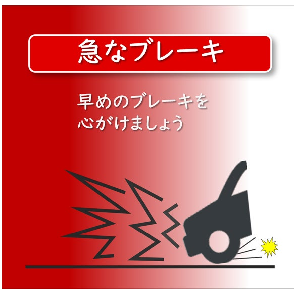
\includegraphics[scale=0.6]{fig/img.pdf}
\caption{Feedback image}
\label{img}
\end{figure}

\subsection{データ収集と選別}
\label{exception}
アンケートのうち,以下の条件に該当する回答を,本発表における解析対象から除外した.
\begin{itemize}
    \item ダミー問題誤答
    \item フィードバック内容の5択問題の誤答
    \item 過去2年以内に運転経験がない人
\end{itemize}
上記の除外基準に基づき,804人(男性431人,女性373人)のアンケート結果を最終的な解析対象とした.

\section{結果及び考察}
\subsection{運転特性(DSQ)}
\label{dsq_l}
\subsubsection{因子分析}
\label{fac}
回答者に共通する運転特性の因子を明らかにするために,運転特性の回答結果を因子分析した.入力データは804人の運転特性に関する18個の質問への回答で,抽出法は最小残差法,回転法はプロマックス回転を採用した.また,因子数決定方法は平行分析に基づき,同じ大きさのランダムなデータで解析を行った平均的な結果より,固有値が大きい因子を採用した.なお,独自性が0.8以上の設問項目は除外した.

因子分析の結果,特徴的な5因子を特定した.
運転特性は,制限速度等などを守り安全確認を慎重に行う『安全運転特性』,気分や悩みなどによって運転がおろそかになる『不安定な運転特性』,自分が事故を起こすことをいつも気にしている『心配性特性』,車がステイタスであると考える『ステイタス特性』,先の信号を見て速度調整をする『事前準備的特性』の5因子が存在することが明らかとなった.

\vspace{\baselineskip}
\subsubsection{クラスタ分析}
\label{clu}
クラスタ分析により運転特性が近しい人同士のクラスタを作成した.
クラスタ分析をするために,運転特性は因子ごとに以下の式(1)を用いて運転特性スコアを算出した.
\begin{equation}
\sum_{Q=1}^{17} (\text{各設問の4件法の値}) \times (\text{各設問の因子負荷量}) \label{eq}
\end{equation}
Q1-17の和を運転特性スコアと定義し,因子ごとに算出することで,それぞれの因子の運転特性を定量化することができる.この際,独自性が0.8以上となった設問を1つ除外したため,17設問の和をスコアとした.

804人分の5因子の運転特性スコア(804×5の配列)を入力し,ウォード法およびユークリッド距離を用いて階層的クラスタリングを行った.
階層的クラスタリングを実施した結果,3クラスタから2クラスタに減少した際のデンドログラムの結合距離の増加が大きかったため,3クラスタが妥当であると判断した.
そして,各クラスタごとに運転特性スコアの平均値を算出した.この結果をFig.\ref{score_d}に示す.

クラスタ1は他のクラスタと比較して有意に不安定な運転特性スコアの値が大きく,心配性特性スコアの値も大きいため,【心配性で不安定な運転傾向の群】と考えられる.同様に,クラスタ2は安全運転特性スコアと心配性特性スコアの値が有意に大きく,不安定な運転特性スコアが有意に小さいため,【心配性傾向はあるが安全運転な群】と考えられる.最後に,クラスタ3は安全運転特性スコアと心配性特性スコアが有意に最も低いことから,【安全運転特性が最も低く,心配性でもない群】と考えられる.

%%%%%%%%%%%%%%%%%%%%%%%%%%%%%%%%%%%%%%%%%%%%%%%%%%%%%%%%%%%%%%%%%%%%%%%%%%%%%%%%%%%%%%%%%
\section{まとめ}
あ

%%%%%%%%%%%%%%%%%%%%%%%%%%%%%%%%%%%%%%%%%%%%%%%%%%%%%%%%%%%%%%%%%%%%%%%%%%%%%%%%%%%%%%%%%
\vspace*{-0.55cm}
\small
\begin{thebibliography}{9}
%%%%%%%%%%%%%%%%%%%%%%%%%%%%%%%%%%%%%%%%%%%%%%%%%%%%%%%%%%%%%%%%%%%%%%%%%%%%%%%
%\bibitem{Influ} Tina Cvahte Ojsterek, Darja Topolek, 2019,  "Influence of drivers’ visual and cognitive attention on their perception of changes in the traffic environment", European Transport Research Review, Article number: 45
%\bibitem{drive_dia}株式会社デンソー,”ドライブレコーダーAI解析技術を活用した高齢者安全運転支援の実証実験”
%\bibitem{drive_t}トヨタ自動車株式会社,”T-Connect My TOYOTA”
%\bibitem{BM1} 深沢 伸幸,1987, ``認知的動機づけの手法を用いた運転行動の変容に関する研究'',産業・組織心理学研究,Vol.1, No.1, pp.29-38
%\bibitem{risk} 大谷 亮, 宇野 宏, 藤田 和男,2007,``交通状況に起因するドライバの危険度過小評価が運転行動に及ぼす影響に関する検討'',日本人間工学会,Vol.43, No.6, p.303-314
%\bibitem{me} 北川 浩行,粕谷 美里,阿部 香澄,2024,"危険運転指摘のための提示手法と運転特性の関連性検証",電子情報通信学会総合大会
%\bibitem{agent} 高田 翔太,平岡 敏洋,野崎 敬太,2013年,”自発的な行動変容を促す安全運転評価システム(第2報)”評価システムが運転行動に与える影響,自動車技術会論文集,Vol.44,No.2,p.673-678
%\bibitem{sub_sys} 島崎 敢,2014,”自分の運転を客観視するための支援システム”,人間工学,Vol.50,No.Supplement,p. S36-S37
%\bibitem{Mul} Ju-Hwan Lee, Charles Spence, 2008, ``Assessing the Benefit of Multimodal Feedback on Dual-Task Performance under Demanding Conditions'', People and Computers XXII Culture, Creativity, Interaction (HCI), Vol.1, pp.185-192
\bibitem{tkt} 永井 正夫,”個人適合型運転診断・支援サービスを搭載した常時記録型ドライブレコーダの開発と行動実証実験(FOT)”
\bibitem{ando} 安藤 章,閔 健熙,2018,”ドライブレコーダーの常時撮影映像等を活用した危険運転発生特性に関する分析”,交通工学論文集,Vol.4,No.1,p.A\_169-A\_176
\bibitem{agent} 藤掛 和広,田中 貴紘,2019年,”ドライバエージェントの運転支援及び振り返り支援による運転行動改善の効果”,自動車技術開論文集,Vol.50,No.1,p.134-141
\bibitem{check} 石橋 基範,大桑 政幸,赤松 幹之,2002,"運転者特性把握のための運転スタイル・運転負担感受性チェックシートの開発'',自動車技術会2002年春季大会学術講演会前刷集,No.55-02,9~12
\bibitem{cog} 本田 真美,"2021,医師のつくった「頭のよさ」テスト~認知特性から見た6つのパターン~",光文社新書
\bibitem{phase} 岡 浩一朗,2003,"中年者における運動行動の変容段階と運動セルフ・エフィカシーの関係",日本公衆衛生雑誌,Vol.50,No.3,p.208-215
\bibitem{p1}Marcus BH, Simkin LR, "The transtheoretical model: Applications to exercise behavior", Med Sci Sports Exerc 1994; 26: 1400-1404
\bibitem{p2}Prochaska JO, Marcus BH, "The transtheoretical model: Applications to exercise", In RK Dishman (Ed.) Advances in exercise adherence. Champaign, IL: Human Kinetics, 1994; 161-180
\bibitem{old_driver} 三村 泰広,樋口 恵一,安藤 良輔,2019,"高齢運転者の運転能力と不安感の関係",土木学会論文集,Vol.75,No.5,p.l\_1103-l\_1112
%%%%%%%%%%%%%%%%%%%%%%%%%%%%%%%%%%%%%%%%%%%%%%%%%%%%%%%%%%%%%%%%%%%%%%%%%%%%%%%
\end{thebibliography}
%
\thispagestyle{fancy}
\renewcommand{\headrulewidth}{0.0pt}

\end{document} 